\begin{frame}{Расчёт ЛТХ}
\begin{block}{В расчёт ЛТХ входит}
   \begin{enumerate}
    \item [] <+->
    \item <+-> Расчёт области возможных полётов
    \item <+-> Расчёт траектории полёта 
    \item <+-> Расчёт транспортных возможностей самолёта
   \end{enumerate}
\end{block}
\end{frame}

\begin{frame}{Расчёт области возможных полётов}

    \begin{block}{Основные ограничения}
        \begin{itemize}
            \item Ограничение по $M_{min \ P}$ 
            \item Ограничение по $M_{max \ P}$
        \end{itemize}
    \end{block}

    \begin{block}{Дополнительные ограничения}
        \begin{itemize}
            \item Ограничение по $C_{y \ \text{доп}}$
            \item Ограничение по $M_\text{пред}$
            \item Ограничение по $q_{maxs}$
        \end{itemize}
    \end{block}

\end{frame}

\begin{frame}{Расчёт области возможных полётов}
    \begin{minipage}[c]{0.55\textwidth}
        \center{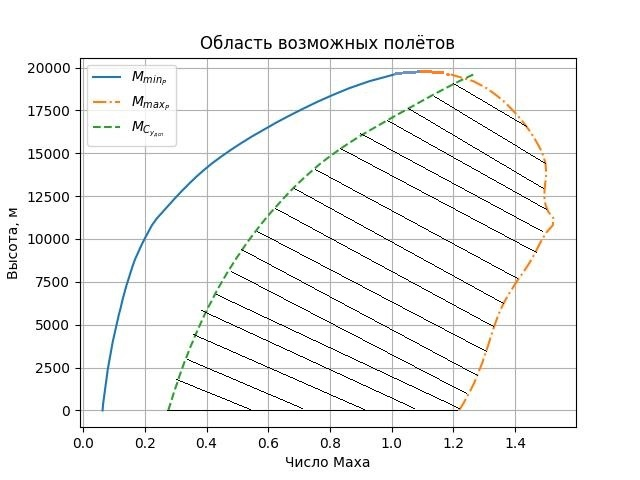
\includegraphics[width=6cm, height = 7cm]{../Оглавление/Part1/figures/Область.jpg}}
    \end{minipage}
    \begin{minipage}[c]{0.4\textwidth}
        \begin{itemize}
            \item <+-> []
            \item <+-> [] \begin{block}{Определение области}
                \begin{itemize}
                    \item $M_{min} = max \{ M_{min \ p}, \ M_{C_{y \ \text{доп}}} \} $
                    \item $M_{max} = min \{ M_{max \ P}, \ M_{\text{пред}}, \ M_{q_{max}} \}$
                \end{itemize}
            \end{block}
        \end{itemize}
    \end{minipage}
\end{frame}

\begin{frame}{Определение теоретического и практического потолка}
    \begin{minipage}[c]{0.45\textwidth}
        \begin{block}{Потолки}
        \begin{itemize}
            \item <+-> []
            \item <+-> [] Расчёт теоретического и практического потолка производится по $V_{y_{max}}$
            \item <+-> [] $H_\text{т} = 19,8$ км 
            \item <+-> [] $H_\text{пр} = 19,5$ км
        \end{itemize}
        \end{block}
    \end{minipage}
    \begin{minipage}[c]{0.45\textwidth}
        \center{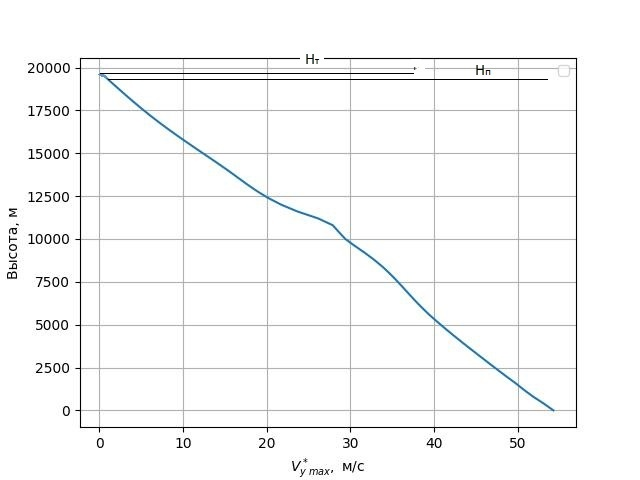
\includegraphics[width=6cm, height = 7cm]{../Оглавление/Part1/figures/Vy(H).jpg}}
    \end{minipage}
\end{frame}

\begin{frame}{Расчёт траектории полёта}
    \begin{block}{Траектория}
    \begin{itemize}
        \item [] <+->
        \item [] <+-> Траеткорию полёта принято разделять на три этапа 
            \begin{itemize}
                \item Набор высоты 
                \item Крейсерский полёт 
                \item Снижение 
            \end{itemize}
    \end{itemize}
    \end{block}
\end{frame}